% Chapter 3

\chapter{Sensibilidad al contexto}
% Write in your own chapter title
\label{Capitulo 3}
\lhead{Capítulo 3. \emph{Sensibilidad al contexto}} % Write in your own chapter title to set the page header

Luego de describir a Seaside como referente para desarrollar aplicaciones web basadas en continuations, es necesario explicar que alternativas existen para procesar la información provista por un conjunto de sensores.

Una forma de organizar la utilización de sensores es mediante el concepto de \emph{sensibilidad al contexto}.

Para poder definir la sensibilidad al contexto es necesario repasar que significa \emph{contexto}, \emph{entorno} y \emph{adaptación}; para luego poder definir la \emph{sensibilidad al contexto}.

%Para comprender la sensibilidad al contexto es importante entender algunos conceptos básicos como el \emph{contexto}, el \emph{entorno} y la \emph{adaptación}.

La primera definición de \emph{contexto}, que es la más adoptada, es la que aporta \emph{Dey} en 2001, que estipula:

\begin{quote}
Contexto es cualquier información que pueda ser usada para caracterizar la situación de una entidad.\cite[p.~3]{Dey01}
\end{quote}

Por su parte, \emph{Dourish} intenta destacar una característica dinámica al intentar abstraer al contexto y en 2004 afirma:

\begin{quote}
Contexto es un concepto de lo que se mantiene al margen, y se disuelve cuando uno intenta definirlo.\cite{Dourish04}
\end{quote}

De esta forma \emph{Dourish} destaca lo complejo que es definir un modelo para representar al contexto, dado que cierta información del contexto puede transformarse en información del modelo y viceversa. Además, presenta un modelo contextual basado en interacciones, que se enfoca en responder ``¿cómo y por qué las personas mantienen un entendimiento mutuo del contexto en el curso de las interacciones de sus acciones?''; evitando así la definición de un contexto \emph{estable} y \emph{delineable} en tiempo de implementación\cite[p.~5]{Dourish04}.

Por otra parte, el \emph{entorno} es la caracterización de las circunstancias de una situación en particular combinado con la descripción de la adaptación a realizarse para mejorar la interacción con el usuario de ese contexto. Es el punto de conexión entre un modelo de negocios y el modelo del contexto, que se encarga de describir ante qué circunstancias se realiza cierta \emph{adaptación}.

Luego, la \emph{adaptación} consiste en realizar un conjunto de acciones de forma automática para simplificar la interacción de una entidad con uno o varios sistemas. Aunque estas acciones sólo afectarán al modelo de negocio, se debe tener en cuenta que cierta información del contexto puede transformarse en información del modelo de negocio y viceversa.

A partir de estos conceptos, se considera que la \emph{sensibilidad al contexto} es una característica de los sistemas que simplifica la interacción con un usuario (o entidad) a partir del \emph{entendimiento} de la situación del mismo (o la misma). Ese \emph{entendimiento} está determinado por la capacidad de un sistema de identificar un \emph{entorno} y luego proporcionar una \emph{adaptación}.

A continuación, dado que la sensibilidad al contexto se encuentra estrechamente relacionada con los sistemas adaptativos, se definen a las \emph{aplicaciones adaptativas sensibles al contexto} de \emph{Efstratiou}\cite{Efstratiou04} para delinear el alcance de esta tesis. Luego, se introducen los conflictos que existen cuando se procede a combinar la sensibilidad al contexto con un framework de aplicaciones web basado en continuations.


\section{Aplicaciones adaptativas sensibles al contexto}

Los sistemas adaptativos\cite{Cen97,Kokar99,Meng01} están basados en la teoría del \emph{control mediante la retroalimentación}\footnote{Utilizado por primera vez en la ingeniería electrónica.} (ver Figura \ref{FeedbackControlSystem}).

\begin{figure}[ht!]
\centering
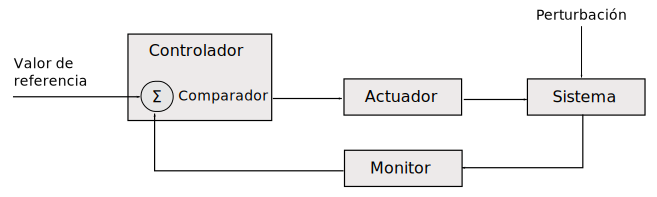
\includegraphics[scale=0.75]{FeedbackControlSystem}
\caption{Sistema de control mediante la retroalimentación}
\label{FeedbackControlSystem}
\end{figure}

El \emph{controlador}\footnote{Este es el \emph{controlador} de la adaptación y no se encuentra directamente relacionado con el controlador del MVC.} se encarga de mantener el valor de referencia de una variable de control, mientras reduce la sensibilidad del sistema a posibles perturbaciones. El controlador interactúa con el sistema a través de \emph{monitores} y \emph{actuadores}.

Un monitor mide la variable controlada, y es la fuente de retroalimentación. La salida del controlador causa que el actuador realice la adaptación al comportamiento del sistema en respuesta a las perturbaciones (o cambios en el entorno).

La abstracción de este sistema puede sintetizarse en un \emph{ciclo de adaptación básico} (ver Figura \ref{BasicAdaptationCycle}) que incluye los siguientes elementos funcionales:

\begin{figure}[ht!]
\centering

\includegraphics[scale=0.75]{BasicAdaptationCycle}
\caption{Ciclo de adaptación básico}
\label{BasicAdaptationCycle}
\end{figure}

\begin{description}
\item[Monitor:] El primer elemento realiza el monitoreo de una fuente de información específica que es \emph{interesante} para el mecanismo de adaptación. Esta fuente de información puede estar determinada por la disponibilidad de un recurso específico o un \emph{disparador contextual} que notifique la ocurrencia de un evento.
\item[Controlador:] El segundo elemento es el mecanismo de control que toma las decisiones necesarias para adaptarse al entorno. Esta decisión se basa en la información recibida por el monitor.
\item[Actuador:] El tercer elemento es el encargado de realizar la adaptación mediante la ejecución de acciones correctivas, a medida que el controlador lo disponga. La conexión entre el actuador y el recurso que está siendo monitoreado no necesariamente existe en todos los sistemas.
\end{description}

\emph{Efstratiou}\cite{Efstratiou04} destaca que una \emph{aplicación adaptativa} adquiere la característica de ser \emph{sensible al contexto} cuando la información a ser monitoreada, en lugar de provenir de un recurso específico, proviene del \emph{contexto externo} de la aplicación (cualquier porción de información que actualmente no pertenezca al \emph{modelo de negocio}).


\section{Conflictos entre la sensibilidad al contexto y las aplicaciones web desarrolladas con continuations}
\label{Conflictos entre sensibilidad y aplicaciones web}

Al comenzar a combinar las aplicaciones web basadas en continuations con técnicas utilizadas por las aplicaciones adaptativas sensibles al contexto surgen dos situaciones de conflicto: la \emph{privacidad} y las \emph{transacciones con adaptación al contexto}.


\subsection{Privacidad}

Las \emph{aplicaciones web} se ejecutan encapsuladas en el navegador web para proveer de cierta seguridad y privacidad al usuario. Se intenta separar su información privada y el conjunto de dispositivos conectados a una computdadora de las inseguridades que provee una conexión a Internet (o intranet).

Por otra parte las \emph{aplicaciones adaptativas sensibles al contexto} necesitan el acceso a la información privada del usuario y a un conjunto de sus sensores, con el fin de identificar el contexto (o entorno) de forma automática y promocionar adaptaciones que simplifiquen la actividad cotidiana del usuario.

Ante esta situación conflictiva, en donde una de las partes restringe el acceso al sistema y la otra requiere todo lo contrario para funcionar, es importante presentar una solución intermedia que brinde la información suficiente para la adaptación, siempre y cuando el usuario lo desee. En el mas restrictivo de los escenarios, el usuario terminará utilizando una aplicación web convencional en donde no exista sensibilidad al contexto.


\subsection{Transacciones}

Las aplicaciones web basadas en continuations suelen contener flujos de control con soporte para transacciones. Una transacción garantiza que un conjunto de acciones sean ejecutadas de forma consecutiva, y ante algún inconveniente existe un mecanismo de \emph{restauración} para dejar el sistema en el estado previo.

Las transacciones son utilizadas por aplicaciones con ejecuciones concurrentes, en donde se desea evitar la corrupción o inconsistencia de los datos al ser persistidos.

Como contraparte, en las aplicaciones adaptativas, las acciones son ejecutadas a partir de una necesidad de adaptación de un sistema a un contexto dado. Una acción siempre depende del entorno que motivó la adaptación.

En las aplicaciones adaptativas la persistencia de la información suele ser realizada de forma acumulativa, de tal manera que se memorice el progreso de la adaptación a través del tiempo. A partir de estos datos, un sistema evolutivo podría reconocer nuevos patrones de comportamiento de un usuario, y proveer nuevas adaptaciones.

Esto produce que no se necesiten modificar valores previos en los sistemas adaptativos, descartando en gran medida la necesidad de transacciones.

El conflicto entre ambas partes ocurre cuando una transacción de un sistema basado en continuations falla y se desea restaurar el sistema a una versión previa. En los sistemas adaptativos sensibles al contexto la única interpretación que admitiría restablecer los registros a un estado previo es aquella que se produciría si se pudiese retroceder el tiempo y sus consecuentes estados.

Dado que esto es improbable, resulta necesario contemplar una alternativa que permita mezclar las transacciones de continuations con la ``progresividad'' de la sensibilidad al contexto.

Para evitar esta situación, se descarta el análisis de cualquier variante \emph{evolutiva} de sensibilidad al contexto en donde se requiere de este tipo de persistencia y se opta por integrar la adaptación al contexto sobre el framework que administra las continuations.

Esto significa que Seaside, administrará las transacciones (encargandose del estado correspondiente) y luego la sensibilidad al contexto por sobre Seaside reconocerá entornos y le notificará al framework para que ejecute las acciones de adaptación correspondiente.

Estas ejecuciones asociadas a ciertos entornos, podrán deshacerse fácilmente al no persistirse la información perteneciente a la sensibilidad al contexto. Solo se persistirán las consecuencias de las adaptaciones en el modelo de negocio de la aplicación transaccional.